
\section{Extended Synopsis and Scientific Proposal}

%\vspace{-.5em}
%\hrule

%\vspace{1.2em}
Beginning with the 1980's, the computer science community has accepted
that computer programs and logical proofs are made of the same fabric.
They are both based on a rigorous formal language, characterized by a grammar,
and they both rely heavily on tree-like structures for defining their semantics,
via syntax-directed derivations.
By now, it has become widely accepted~\cite{PNAS1934:Curry,Essay1969:Howard,IC1988:Coquand,CACM2015:Wadler} that the task of writing a program can be
reduced to that of finding a proof to a conjecture, and conversely, the task of
proving a theorem can be reduced to producing a program with some specific
characteristics.
In addition to that, logic is at the core of software verification, as a basis
for specifications~\cite{LPAR2010:Leino,ECOOP2013:Regis,ICSE2009:Schulte,PASTE2005:Barnett,CAV2015:Gurfinkel}, loop invariants~\cite{VMCAI2011:Bradley,CAV2013:Komuravelli,CAV2019:Feldman}, rely-guarantee properties for concurrent programs~\cite{relyguarantee1,TCS2007:Jones}, and more.
The task of checking adherence to a program's specification is also reduced, in
more than one way, to deciding the validity of a logical formula.

\medskip
This proposal is based on a fundamental understanding, that breaking existing
barriers in automated reasoning is a key ingredient that will lead to
much more powerful mechanism for the construction of provably-correct software.
By powerful, we mean scalable to the sizes of realistic software modules,
adaptable to arbitrarily complex properties,
and requiring less user effort thanks to an increased level of automation.
To achieve this goal, this research \textbf{aims to bridge the gap between two insofar prevalent automated  reasoning disciplines}:

\begin{paragraph}{Automated Theorem Provers (ATP)} A family of tools and techniques based on proof
theory of logical deduction.
A logic in this setting is characterized by a vocabulary and a system of
inference rules; provers are tasked with searching the space of proofs, which
are essentially trees (more generally, DAGs) constructed from repeated
application of the inference rules.
\end{paragraph}

\begin{paragraph}{Satisfiability-Modulo-Theory Solvers (SMT)} A somewhat newer approach with roots in complexity theory and algorithms for solving the Boolean satisfiability problem (SAT).
These algorithms have been augmented with decision procedures for several first-order fragments.
SMT solvers have become incredibly popular thanks to highly efficient implementations and very successful optimization heuristics that manage to combat the inherent intractability of the problem.
\end{paragraph}

\medskip

%\todo{Merge description of ATP and SMT to the background; write here a short paragraph defining these two things and saying that the idea is to merge them}


%The expected result is a proof leading to a desired statement (closed formula)
%$\varphi$, that can be used as a certificate to the logical validity of
%$\varphi$ --- that is, it can be checked mechanically to confirm the soundness
%of each inference step.
%While proof search can be a very costly process, due to the inherent complexity
%of the search space, checking a proof is usually swift and done with linear
%cost with respect to its size.

\begin{comment}

%\begin{comment}
\todo{remove this from here and put in background, it kills the flow}
It is worth mentioning a third camp, that has, so far, received less
attention from the programming languages and automated reasoning crowd.

\paragraph{CSP Solvers} Constraint Satisfaction Problems (CSP) are ubiquitous
in planning, AI, and various other fields of computer science.
The ultimate goal of CSP is to find parameters that satisfy a set of (mostly
numerical) constraints. The solutions can be useful for scheduling tasks,
motion planning, \etc.
CSP solvers excel at solving puzzles such as the $N$-queen problem or Sudoku.
Their use in automated theorem proving is insofar limited.
\end{comment}

\smallskip
These two camps, coming from such different backgrounds,
face a serious gap in both theory and practice,
one that currently prevents adoption of results from one approach into use in
the other.
The primary goal of this research is to construct a unified framework for automated reasoning, where proving
and solving techniques can cooperate.
Such framework need not be constrained by the boundaries of some specific logic, such as first-order logic or linear integer arithmetic.
Instead, careful parameterization will allow adaptive treatment of a wide spectrum of domains, where existing techniques can be seen as individual points in the more general space.
This will allow to leverage the power of ATP and SMT into proving the more complex
conjectures required for software verification and synthesis.
When it comes to applying SMT, one major obstacle in many problem domains, is
that SMT solvers are generally restricted to first-order logic; at the same time,
the properties one wishes to prove require reasoning about composite structures (such as lists, maps, and streams), and, most often, the use of induction.
Theorem provers can more easily be equipped with higher-order logic and induction-oriented inference
rules.
Still, sub-problems arising in the course of resolving the induction step can
and should benefit from honed SAT and SMT capabilities.

As an overarching goal, this research will \textbf{lay foundations for a new discipline
in automated provers, by way of integrating the camps of ATP and SMT and allowing
cross-fertilization}.
Specifically, it is motivated by provers for the tasks of software verification
and synthesis; these are characterized by relying almost exclusively on discrete
mathematics, such as set theory, graphs, automata, an algebraic construction of
natural numbers, and various theories of integer arithmetic.


\subsection{Background}

%\todo{The background should put an emphasis on what each tool is good at}

\begin{paragraph}{Automated Theorem Provers}
Proof theory is a branch of logic that has gained much traction in the 20th century with the advent of Hilbert~\cite{Book1928:Hilbert} and Gentzen~\cite{j1935:Gentzen},
both of whom developed calcli for algorithmic formalization of proofs.
As computers became available, it was natural that these notions be implemented as programs.
As early as 1960~\cite{Wiley1960:Wang,Wiley1961:Wang}, large automatic systems for theorem provers have been used by the research community for a variety of logical reasoning tasks.
Most of these early systems were based on the resolution principle~\cite{JACM1965:Robinson}, which continues to be popular today.
Term unification~\cite{IJCM1965:Robinson} is used to resolve first-order formulas.
In the 1990's, superposition calculus~\cite{LPAR1992:Bachmair} emerged as the leading technique for equality reasoning.
This led to several successful theorem provers, notably Vampire~\cite{JAR1995:Voronkov,CAV2013:Kovacs}, E prover~\cite{AIC2002:Schulz}, and iProver~\cite{CADE2008:Korovin}.
Today, most theorem provers rely in one way or another on term rewriting for the implementation of superposition, based on the Knuth-Bendix algorithm~\cite{AR1983:Knuth} for normalizing rewrites.

More recently, a lot of attention was directed towards \emph{cyclic proof systems}, a form of Gentzen-style calculus that natively admits proof by induction.
Instead of the traditional induction scheme or induction rule, \eg (for $\mathbb{N}$) $P(0)\land \forall k.\,P(k)\to P(k+1) \vdash \forall n.\,P(n)$,
cyclic proofs admit ancestor sequents as premises to a later inference steps --- thereby allowing the proofs to contain cycles.
To avoid unsoundness caused by a self-referencing statement, cyclic proof systems impose a \emph{global trace condition} that ensure cycles cannot be unrolled \textit{ad infinitum}.
This trace condition is carefully crafted for every cyclic system to enable a soundness proof for the system.
In a way, whatever complexity is removed from the proof proper is shifted to the global trace condition;
however, this allows for some pretty sophisticated trace conditions, such as those based on B\"uchi automata.
In turn, these allow such systems to provide exetremely succinct and elegant proofs.
\end{paragraph}

\begin{paragraph}{Satisfiability-Modulo-Theory Solvers}
A somewhat newer approach is based on extending the
Boolean satisfiability problem (SAT) with first-order theories and arithmetic, leading to
Satisfiability Modulo Theory (SMT).
SAT solvers accept Boolean formulas and construct a satisfying assignment, or
declare that none exists.
Since SAT is NP-complete (in fact, usually referred to as \emph{the} canonical
NP-complete problem), finding the solution may be time consuming, but eventual
termination is guaranteed.
SMT solvers take first-order formulas and attempt to find a first-order
\emph{model} for them, that is consistent with an underlying theory --- where the
theory is built into the solver.
The theories generally put no bound on the size of the models they admit
(\eg, numerical theories are typically defined over the domain of integers),
and as expected, the problem is generally undecidable.
However, despite the inherent complexity of SAT and undecidability of SMT,
solver technology has become extremely successful, especially in applications
relating to software verification.
In this context, proving a verification condition (``theorem'') $\varphi$
amounts to finding its negation $\lnot\varphi$ unsatisfiable --- which is the root
of the connection, and contention, between SMT solvers and theorem provers.
For many software verification conditions, SMT solvers have been shown to be
more effective in proving the validity of verification conditions than
contemporary proof theory-based theorem provers.

SAT and SMT received much tractions in the Model Checking community~\cite{Book2001:Clarke,SSS2014:Grumberg} thanks to their successful applications to formal methods.
SAT was initially utilized for hardware verification of logical circuits, and SMT became a natural extension for dealing with software, as programming languages typically provide primitives such as integer values~\cite{CAV2006:Dutertre}, bit vectors~\cite{TACAS2007:Bryant}, and arrays~\cite{CAV2007:Ganesh}.
Because loops are pervasive in both hardware and software systems, there is an ever-present need for reasoning about executions of unbounded length.
To that end, \emph{loop invariants} play a crucial role in all software verification systems~\cite{LPAR2010:Leino,PLDI2016:Padon,ECOOP2013:Regis}.
This essentially facilitates an induction scheme, but, by and large, the burden of supplying the invariant remains with the programmer.
\emph{Invariant inference} is a big open problem that stands in the way to effective software verification.
A significant breakthrough in invariant inference was achieved last decade with the development of the IC3 algorithm~\cite{VMCAI2011:Bradley} for automatic inference of Boolean invariants for hardware model checking.
This sprouted a line of successful follow-up works on Property-Directed Reachability~\cite{VMCAI2015:Bjorner,CAV2016:Fedyukovich,CAV2014:Vizel,VMCAI2017:Vizel,CAV2019:Shemer}.
These results have been integrated into the leading SMT solver Z3~\cite{Z3SMT,CAV2013:Komuravelli,CAV2014:Komuravelli} and constitute key components of the SeaHorn verifier~\cite{TACAS2015:Gurfinkel} for C programs.
\end{paragraph}


\subsection{Research Objectives and Methodology}

%\todo{Be more specific about the problems and why they are important: e.g. "cope with Boolean constructs", "unavoidable in software verification" etc.; explain what gives rise to these instances}

\begin{paragraph}{Objective 1: {\it Bridging equality and congruence}}~
Equality and equivalence are fundamental terms in mathematics and computer science.
Therefore, equality is a native primitive in most logics.
SMT solvers rely on a decision procedure for (quantifier-free) congruence closure together with the Nelson-Oppen method for combining it with other theories~\cite{JACM1980:Nelson}.
ATPs, by and large, are invested in superposition calculus, which is driven by term rewriting.
To support efficient rewriting and avoid backtracking, modern ATPs such as Vampire and E employ an order relation on terms, so that all rewrites are directed.
Both of these approaches limit the provers' ability to reason about equalities given as assumptions or discovered as conjectures in the course of the search:
This is due to the quantifier-free nature of Nelson-Oppen, leading to a constant need for speculative quantifier instantiation, on one hand;
and the requirement for ordering, which relies on the Knuth-Bendix algorithm, which in turn is incomplete --- so it cannot be expected to produce a normalizing ordering for an arbitrary set of univerally-quantified equalities that has been accumulated.
We propose, as a unifying mechanism, to further utilize the notion of \emph{equality graphs} (e-graphs), as is done in some SMT solvers~\cite{IC2007:Nieuwenhuis,CADE2007:deMoura,TACAS2017:Barbosa} for performance purposes.
We combine this with term rewriting and \emph{equality saturation} to obtain \emph{unordered} sets of equivalence terms (e-classes).
E-graphs are known to be space-efficient by reducing duplication in the representation of terms to a minimum, employing congruence closure as a core mechanism to merge class nodes and keep the graph compact.
This knowledge is maintained as part of the prover's state and can be updated incrementally when the prover discovers new conjectures.
To cope with Boolean constructs (such as implications and disjunctions, which are frequent in verification conditions due to the presence of branching statements in programs), we propose a novel solution, \emph{e-graph coloring}, by which sub-components of the e-graph can be annotated with certain ``colors''; the colors denote that the validity of some propositions is subject to one or more assumptions, in the spirit of Gentzen's sequents.
This enables the use of assumptions similar to how they are introduced in CDCL(T), with easy backtracking when a conflict occurs.

This will lay a foundation in which e-graphs are the glue that binds SMT-style equality reasoning, that is based on congruence, and the ATP-style superposition, without requiring terms to have a normal form, and while incorporating the power of SAT in handling Boolean conditions and predicates.
\end{paragraph}

\begin{paragraph}{Objective 2: {\it Bridging induction}}~
The success of SMT solvers with first-order reasoning led to their wide adoption in software verification.
This gives rise to the challenge of representing unbounded state (\eg size of data structures) and unbounded time (\eg number of loop iterations).
The proposed framework will try to generalize and unify the two leading frontiers for reasoning by induction.
In the world of model checking and SMT, the IC3 algorithm and its variants %~\todo{remember to cite them in the background}
has proven to be the gold standard for automatic invariant inference.
In proof theory and deductive reasoning, cyclic proof systems provide shorter proofs, which have good value for ATPs such as Cyclist, where proof search is severely limited by the depth of the proofs that can be feasibly explored.
These two approaches to proof by induction are vastly different: IC3 is counterexample-driven; Cyclist is proof-driven.
We plan to draw on the duality between reachability and invariant inference~\cite{arXiv2020:Padon} to create a unified description of the two processes, where both aspects, inductive and deductive, will manifest.
This new setting would allow the conclusions accumulated with the IC3 method to direct and guide the proof search, and intermediate conclusions from closed cycles in the pre-proof being constructed to inform the clause inference that is a core step of IC3.

More broadly, IC3 can be seen as a process where a proposition is repeatedly \emph{strengthened} until it becomes inductive and can be used as an inductive loop invariant.
Constructing a proof can also be seen as starting with a proof goal and strengthening it by choosing (a set of) subgoals that entail it.
On the other hand, both processes have crucial elements of \emph{weakening} as well: in IC3, a single counterexample (represented as a \emph{cube}, \ie, a conjunction of literals) needs to be generalized in order to ``block'' an entire set of unreachable states.
This is essential to IC3's good performance relative to more traditional model checking.
In deductive proof search, \emph{cuts} are required to support the construction of proofs by case analysis.
Each case represents a conjecture that is weaker than the general proposition, and knowing which  cases to create is known to be a pain point in automated deduction.
We plan to use partial solutions from over-approximation of the set of reachable ``states'' (representing logical structures) to assist in pruning a deductive proof search process and as a way to suggest conjectures that can be used in case analysis.
Conversely, sequents inferred during proof search can be used in generalizing counterexamples as part of the ``block'' phase of IC3, leading to more effective generalizations and better convergence properties.

To allow seamless information exchange between these frameworks, we propose a method for putting them on a common mathematical foundation.
We draw inspiration from~\cite{Book2003:Avron}, where it was shown that all instances of finitary induction, \ie, induction over countable domains, can be captured by FO(TC) --- first-order logic extended with \emph{transitive closure}.
TC provides a good middle ground for combining induction strategies because
(i) it naturally captures the notion of reachability around which IC3 is built, and
(ii) it has been successfully formulated within the cyclic proof framework~\cite{TOCL2020:Cohen}.
Moreover, the latter also facilitates coinduction~\cite{IJCAR2020:Cohen}, which allows proofs over infinite traces (\ie, non-terminating executions) and streams of input.
This may give rise to a new adaptation of IC3 to coinduction, which has not been proposed until now.

State-of-the-art software verification tools such as SeaHorn~\cite{TACAS2015:Gurfinkel} employ an intermediate representation of the verification task as a system of Constrained Horn Clauses (CHCs) %\todo{make sure these are mentioned in the background} 
and apply IC3 in order to solve them.
An interesting problem in CHC solving arises when clauses are \emph{non-linear}, that is, the body (left-hand side of the implication) of the rule contains more than one uninterpreted literal.
A similar problem arises in reasoning with TC logic when trees (rather than chains, or sequences) are involved.
Both require handling \emph{branching} paths during exploration.
Combining partial results from both disciplines will provide a more complete solution to this problem,
and improve our understanding and treatment of branching induction in proofs.

%\todo{say here: IC3 is good at finding invariants and the like, cyclic proofs are good at [other things], therefore...}

%\todo{IC3 is counterexample-driven; Cyclist is proof-driven. We plan to draw on the metioned duality to construct a tool that maintains and over- and under-approximation of the space of states/logical structures}
%\todo{use a generalized framework: - use cyclic proof search to locally block counterexamples; - use discovered clauses and/or models to prune some branches early, or, conversely, strengthen some hypotheses to make them inductive based on the relative inductiveness of clauses in IC3 frames}
\end{paragraph}


\begin{paragraph}{Objective 3: {\it Combining proof techniques through modular reasoning}}
For an automated reasoning task of any scale beyond trivial, decomposing goals into sub-goals that can be solved independently is an invaluable tool.
This is especially true when it comes to software verification, and the need for it is only emphasized by broadening the scope of acceptable logics and theories.
Putting in mind that a unified framework for automated reasoning strives to combine together proof strategies of several existing tools,
it is even more challenging --- but also potentially more beneficial --- to ``divide and conquer''.
This would increase the flexibility in applying different strategies and automatically turning some exploration features on or off, selectively.
It provides one way of mitigating the risk involved in a more expressive proof system, allowing to take bolder decisions for inclusion of certain inference tactics.

\begin{wrapfigure}[8]{r}{4.5cm}
\vspace{-1em}
\begin{tikzpicture}
\node(plant)[inner sep=0]{
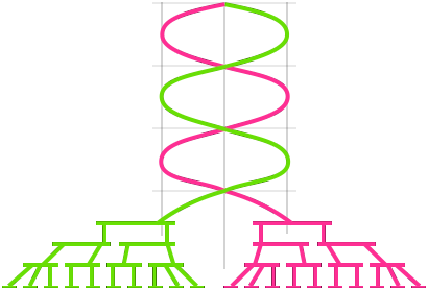
\includegraphics[width=4.5cm]{img/untangled}
};
\node[align=center, yshift=1.4em, anchor=east,
      font=\fontsize{8pt}{8pt}\selectfont]
      at (plant.east) {untangle\\ phase};
\node[align=center, yshift=-1.5em, anchor=east,
      font=\fontsize{8pt}{8pt}\selectfont]
      at (plant.east) {conquer\\ phase};
\end{tikzpicture}

\end{wrapfigure}

In a traditional top-down proof search based on a system of inference rules, the prover must reach the system's \emph{axioms} --- rules with no logical premises ---
in order to seal off a proof branch.
Only following successful closure of all proof branches can the prover declare victory.
Two major factors contribute to search-space explosion:
the proof \emph{width}, caused by having multiple rules be applicable at any given point in the proof;
and proof \emph{depth}, caused by the long chain of rules that have to be applied, consecutively, in order to reach the axioms from the proof goal.

%\todo{The key ingredient here is that when searching top-down, you need to reach axioms in the leaves; when combining bottom-up, you can stop earlier when you have reached a lemma that was discovered previously.
%More importantly, the lemma can be discovered by a variety of proof techniques, which can be SMT- or ATP-driven.}
Our modularization approach for more effective theorem proving is based on the introduction and use of \emph{ancillary lemmas}, encapsulating some details of the proof and reducing the search depth by providing a wider range of known facts that can be used as leaves.
Such lemmas are typical in mathematical pen-and-paper proofs, and they are layered on top of one another to be able to convey a complex development.
To amplify the significance of lemmas we propose a novel approach to problem decomposition, called \textbf{untangle-and-conquer}.
As the name suggests, it consists of two phases, the first of which is aimed at splitting a proof goal such that each sub-proof can be comfortably completed using an existing database of lemmas.
We identify the following gap: logical propositions occurring as proof goals contain a mixture of logical symbols from different theories.
For example, they may contain operations on arrays as well as linear arithmetic over the indices and pointer operations on the elements.
In contrast, lemmas are naturally smaller and involve only a handful of symbols.
This applies to both human-constructed lemmas, because the cognitive load required to deal with intricate interactions between too many different concepts is high;
and to automatically generated lemmas (which we discuss shortly), since large vocabularies incur high resource costs to search through.
It is therefore desirable to engineer the proof in such a way, that each part contains a subset of the symbols occurring in the goal.


Oftentimes, choosing the right lemmas to use as stepping stones is the key insight a mathematician has to come up with.
It would definitely be presumptious to expect an automated reasoning program to replicate this much insight; but there are two key factors working to our advantage when dealing with software-oriented proofs:
(i) Even if some lemmas require ingenuity in their formulation, there is an even larger number of simpler, more ``mundane'' lemmas, and finding those automatically removes tedium from the human user;
(ii) Lemmas used in different proofs are often similar, 
so building a database of discovered lemmas can help the prover in future endeavors;
(iii) By the same argument, using a corpus of previously completed proofs (either human- or machine-generated) can guide the search for lemmas and make use of past results.

We are especially interested in \emph{theory exploration} (or \emph{theory forming}):
Given a library of proven properties, an automated reasoning system can eagerly search for consequences, thereby growing the body of ``knowledge'' at the prover's disposal.
Deductive proof search in ATPs such as Vampire and Cyclist tends to be oriented ``top-down'', that is,
starting from a proof goal, simplifying it further and further until axioms are reached.
The is analoguous to building the proof tree from the root down to the leaves. (Although, graphically, proof trees are commonly depicted with the root at the bottom --- this is nevertheless a top-down approach.)
The availability of synthesis technology \cite{JFP2017:Smallbone,ITP2017:Johansson,arXiv2020:Singher} means that we can generate a vast number of lemmas to guide our untangle-based decomposition.
My premiliminary results from developing TheSy~\cite{arXiv2020:Singher}, a framework for synthesizing lemmas, show that by generating many lemmas and proving them, individualy, by induction, it is possible to prove theorems that previously required the use of an SMT solver (CVC4~\cite{VMCAI2015:Reynolds}), using a relatively modest procedure of congruence closure.
This is a very encouraging and promising direction.

A major risk in doing so is that too many lemmas may incur a high overhead and, moreover, produce too many different ways to decompose a given proof.
We propose to mitigate this by developing a ranking method for discovered lemmas based on their usefulness,
so that our automated reasoning tool can \textbf{learn from experience} and get better over time, using classic statistical inference.
\end{paragraph}

\begin{paragraph}{Objective 4: {\it Extrapolating to Software}}~
The overarching goal of this research is to pave the way for the next generation of theorem proving technology.
The emphasis remains on making tools that allow reasoning about properties of computer programs.
What this means is that an automated prover is required to cope with a high volume of low-level details that interact in unexpected ways.
We would like to take advantage of \textbf{inherent abstraction layers} that already exist in software,
since abstraction is what makes it possible
for human programmers to cope with its ever-growing complexity.
One form of abstraction can be used via the ancillary lemmas described above.
An orthogonal axis is the application of \textbf{semi-automatic refinement} to provide encapsulation for some of the implementation details.
For example, an ordered data structure may be abstracted as a set and a (total or partial) order relation; a multi-threaded process may be abstracted as a sequential one that is behaviorally equivalent.
Choosing the abstraction to use in a refinement proof would, more often than not, require some human intuition, which is why some amount of user interaction will be needed.
With the right abstraction in place,  the automated prover will be able to carry out all or most of the refinement proofs,
showing that the abstraction soundly models the underlying implementation and also inferring system invariants from it --- making this process extremely rewarding.

I will focus on the incorporation of Separation Logic and its modern variants such as Iris~\cite{iris} for modeling a program's memory, \esp in programs that use dynamic allocation or multiple threads with shared state.
In essence, what Separation Logic provides is a refinement that \textbf{correlates the low-level, imperative, mutable semantics of pointer programs with high-level, functional, immutable semantics} that are closer to mathematical definitions.
The increasing popularity of SL dialects for describing complex properties such as object ownership and thread synchronization provides a natural form of ``embedded'' abstraction:
Because SL propositions rely heavily on inductive definitions, the functional interpretation emerges from the specifications.
Establishing the correlation, then leveraging it to prove properties of the underlying program, is a fine example of proof modularization.
The pillars of equality reasoning and proof by induction are both central in this effort.

I will draw on results from my work on \textsc{Cypress}~\cite{PLDI2021:Itzhaky}, a system for synthesizing programs from specifications given in Separation Logic.
\textsc{Cypress} heavily utilizes the concept of cyclic proofs and project it onto the program space,
to facilitate synthesis of recursive auxiliary procedures.

I will also perpetuate my efforts to reason about unbounded-state software systems via a combination of \emph{induction over time} (number of loop iterations or recursive calls) and \emph{induction over space} (size of data structures in a program's memory)~\cite{VMCAI2020:Ish-Shalom,ESOP2021:Ish-Shalom}.
This work introduced \emph{state squeezers}, an alternative induction scheme based on a well-founded ordering of program states.
They have already been applied successfully to verification of challenging safety properties and to automatic inference of complexity bounds that were beyond reach for existing analysis systems.
\end{paragraph}


\begin{comment}
% I am not sure what to do with this
Another obstacle, which hinders both approaches, is the use of quantification
in assumptions and theorems.
One generally wishes to take advantage of the inherent modularity in proving
most kinds of properties, be those mathematical theorems in algebra or combinatorics,
and definitely when it comes to correctness properties of computer programs.
Software is modular by nature, 
It is very much desirable to adopt the same contributing factor to reasoning about
these programs.
This means that instead of constructing one monolithic proof of the ``ultimate
theorem'', one identifies and proves \emph{lemmas} that abstract and generalize
domain knowledge and understanding of the underlying program --- layering them
up until the final goal is met.
This is definitely how it is done in academic papers, and, more recently, in
large software verification projects.
Going back to the challenge at hand, these auxiliary lemmas typically include
quantified formulas, which are logic's way of expressing generalized conjectures.
Applying these lemmas, \eg in the context of carrying out the next step of the proof,
ultimately requires to instantiate universal quantifiers with logical terms.
Since the space of available terms is large (or even infinite), this becomes
a task that is daunting to automate and requires the employment of heuristics
to select the right instances.
We will move to consolidate instantiation strategies into ones that more closely
matches the search for proof --- thus being goal-directed rather then origin-directed.
A primary aim is to make these strategies less heuristic and more predictable.
\end{comment}


\subsection{Impact and Evaluation of Project Success}

My earlier work~\cite{CAV2013,POPL2014,CAV2014,PLDI2014,ICDT2017} and some follow-up by others~\cite{OOPSLA2017:Padon,VMCAI2017:Frumkin,PLDI2018:Taube,CAV2019:Berkovits,CAV2019:Feldman} revolved around the use of decidable logics to encode verification conditions for software,
and transferring these to an SMT solver.
These decidable fragments are extremely limited, and once you ``cross the line'' of undecidability, performance is largly unpredictable.
There are many practical solvers that are able to prove many naturally occurring problems with arithmetic, arrays, and lists;
but pile up too many undecidable particles on top of one another, and frequent divergence ensues, with little to no recourse for debugging the cause.

Automated theorem provers piorneered and play a crucial rule in computerized formalization of mathematics.
So far, they have taken the back seat when it comes to software verification and synthesis.
This is about to change.
The inclination of SMT solvers to integrate concepts of induction~\cite{VMCAI2015:Reynolds} and higher-order reasoning~\cite{smt-from-matryoshka} on one hand,
and the renewed success of ATPs in core PL areas such as Separation Logic on the other,
mark the dawn of a new era in which ATP and SMT come together and join forces.

The Matryoshka project~\cite{what} set as their target to enrich SMT solvers with higher-order constructs such as recursive definitions and second-order quantification.
Although this allows for a more natural, straightforward encoding of software-related queries, there is very much a glass ceiling imposed by the SMT core.
Instead, this project's aim is to inspire a \textbf{paradigm shift} in prover design, putting less focus on fine-tuned heuristics to cover an ever-increasing set of benchmarks, and diverting more effort to \emph{transparency and comprehensibility} of the results.
Generating short, readable proofs, as well as interpretable explanations in cases of failure to find a proof,
are key to mitigate of the risks and remove of the element of dread that accompanies usage of contemprary ATPs and SMT solvers.
In addition, careful regression experiments that will ensure that our team will not have to reinvent existing technology, but build on the vast experience of the past decades of research.
